\documentclass[]{article}
\usepackage{lmodern}
\usepackage{amssymb,amsmath}
\usepackage{ifxetex,ifluatex}
\usepackage{fixltx2e} % provides \textsubscript
\ifnum 0\ifxetex 1\fi\ifluatex 1\fi=0 % if pdftex
  \usepackage[T1]{fontenc}
  \usepackage[utf8]{inputenc}
\else % if luatex or xelatex
  \ifxetex
    \usepackage{mathspec}
  \else
    \usepackage{fontspec}
  \fi
  \defaultfontfeatures{Ligatures=TeX,Scale=MatchLowercase}
\fi
% use upquote if available, for straight quotes in verbatim environments
\IfFileExists{upquote.sty}{\usepackage{upquote}}{}
% use microtype if available
\IfFileExists{microtype.sty}{%
\usepackage{microtype}
\UseMicrotypeSet[protrusion]{basicmath} % disable protrusion for tt fonts
}{}
\usepackage[margin=1in]{geometry}
\usepackage{hyperref}
\hypersetup{unicode=true,
            pdftitle={Does oil price volatility scale with oil price?},
            pdfauthor={James Hamski (james.hamski@spsmail.cuny.edu)},
            pdfborder={0 0 0},
            breaklinks=true}
\urlstyle{same}  % don't use monospace font for urls
\usepackage{longtable,booktabs}
\usepackage{graphicx,grffile}
\makeatletter
\def\maxwidth{\ifdim\Gin@nat@width>\linewidth\linewidth\else\Gin@nat@width\fi}
\def\maxheight{\ifdim\Gin@nat@height>\textheight\textheight\else\Gin@nat@height\fi}
\makeatother
% Scale images if necessary, so that they will not overflow the page
% margins by default, and it is still possible to overwrite the defaults
% using explicit options in \includegraphics[width, height, ...]{}
\setkeys{Gin}{width=\maxwidth,height=\maxheight,keepaspectratio}
\IfFileExists{parskip.sty}{%
\usepackage{parskip}
}{% else
\setlength{\parindent}{0pt}
\setlength{\parskip}{6pt plus 2pt minus 1pt}
}
\setlength{\emergencystretch}{3em}  % prevent overfull lines
\providecommand{\tightlist}{%
  \setlength{\itemsep}{0pt}\setlength{\parskip}{0pt}}
\setcounter{secnumdepth}{5}
% Redefines (sub)paragraphs to behave more like sections
\ifx\paragraph\undefined\else
\let\oldparagraph\paragraph
\renewcommand{\paragraph}[1]{\oldparagraph{#1}\mbox{}}
\fi
\ifx\subparagraph\undefined\else
\let\oldsubparagraph\subparagraph
\renewcommand{\subparagraph}[1]{\oldsubparagraph{#1}\mbox{}}
\fi

%%% Use protect on footnotes to avoid problems with footnotes in titles
\let\rmarkdownfootnote\footnote%
\def\footnote{\protect\rmarkdownfootnote}

%%% Change title format to be more compact
\usepackage{titling}

% Create subtitle command for use in maketitle
\newcommand{\subtitle}[1]{
  \posttitle{
    \begin{center}\large#1\end{center}
    }
}

\setlength{\droptitle}{-2em}
  \title{Does oil price volatility scale with oil price?}
  \pretitle{\vspace{\droptitle}\centering\huge}
  \posttitle{\par}
  \author{James Hamski
(\href{mailto:james.hamski@spsmail.cuny.edu}{\nolinkurl{james.hamski@spsmail.cuny.edu}})}
  \preauthor{\centering\large\emph}
  \postauthor{\par}
  \predate{\centering\large\emph}
  \postdate{\par}
  \date{May 2017}


\begin{document}
\maketitle

\section{Introduction}\label{introduction}

In a commodity trading market the price level is expected to be tied to
commodity system dynamics, namely supply, demand, and delivery of the
commodity being traded. Volatility, the variation in price over time,
reflects uncertainty in the balance of these system factors. This
research paper aims to answer a simply posed question: ``does oil price
volatility scale with price?''; i.e., can we expect to observe larger
price swings when the price is near \$100 per barrel vs \$20 per barrel?

If oil price volatility reflects uncertainty about supply and demand
dynamics, it isn't immediately clear whether we should expect volatility
to depend on price level. Higher oil prices are associated with
``tightness'' in the supply market, meaning there is little excess
capacity to increase production, therefore we may expect swings higher
but some base price support that results in lower measured volatility.
Likewise, low prices may suggest excess capacity that can buffer shocks
to the oil delivery system, dampening volatility. Despite these ``just
so'' arguments, a multitude of factors such as storage dynamics, supply
chain disruptions, the ability of producers to increase production to
bring more oil to market or shut in production capacity in response to
prices (``rebalancing''), and market speculation complicate this picture
and suggest it must be studied empirically.

If it is found that oil price volatility is dependent on price level,
the relationship may follow a scaling formula. For instance, if we can
expect volatility of \$1/barrel when oil is at \$20/barrel, can we
expect volatility of \$5/barrel at \$100/barrel price levels via a
simple linear scaling rule? Three methods are presented in this research
paper to answer this question: (1) regression modeling of price and
volatility, (2) viewing volatility within oil price regimes, and (3)
using multivariate Generalized Autoregressive Conditional
Heteroskedasticity (GARCH) modeling.

Note that in this research paper \emph{oil price} is used to
specifically mean spot-traded crude oil. This represents only one
component of the oil markets, and most of the actual oil price is
determined by futures and long term delivery contracts (need cite). This
research paper is concerned with understanding the energy system using
pricing information. In this way, it differs from much of the published
research in that it is not concerned with forecasting prices or
volatility. Nor is it addressing exogeneous system elements such as
equity markets or interest rates, though the literature shows that the
crude oil market and larger economic indicators are intertwined (add
cite). Instead, it contributes to our understanding of the system
dynamics of an essential energy commodity.

\section{Exploratory Data Analysis}\label{exploratory-data-analysis}

\subsection{Data Source}\label{data-source}

The data source is the West Texas Intermediate (WTI) nominal (i.e.~not
inflation adjusted) daily spot price record from the U.S. Energy
Information Administration. Using nominal prices maintains the ability
to assess volatility for a given time period without introducing an
exogenious factor via inflation adjustment. The WTI series was filtered
to the date range January 2, 1986 through December 30, 2016 (Table 1).

\begin{longtable}[]{@{}lll@{}}
\caption{Oil price series date and price ranges.}\tabularnewline
\toprule
& Date Range & Price Range\tabularnewline
\midrule
\endfirsthead
\toprule
& Date Range & Price Range\tabularnewline
\midrule
\endhead
& Min. :1986-01-03 & Min. : 10.25\tabularnewline
& 1st Qu.:1993-09-01 & 1st Qu.: 19.38\tabularnewline
& Median :2001-06-11 & Median : 28.01\tabularnewline
& Mean :2001-06-19 & Mean : 42.87\tabularnewline
& 3rd Qu.:2009-03-31 & 3rd Qu.: 63.47\tabularnewline
& Max. :2016-12-30 & Max. :145.31\tabularnewline
\bottomrule
\end{longtable}

\subsection{Returns and Volatility}\label{returns-and-volatility}

In this research paper, volatility is characterized two ways: (1) 5-day
historic volatility and (2) 30-day historic volatility. Historic
volatility is defined as: \[V_{H,t}=\sqrt{N}sd(P)\]

In addition, the relationship between the returns themselves and price
level is investigated. Daily returns were calculated as:
\[R_t = \ln({P_t-P_{t-1}})\] Note that the standard return formula takes
the log of the daily price differences, meaning the day to day price
differences are scaled using a natural logarithm. In some sections, the
absolute value of ``unscaled returns'' (i.e. \(|P_t-P_{t-1}|\)) are used
in order to investigate the scaling of the return series.

\begin{figure}[htbp]
\centering
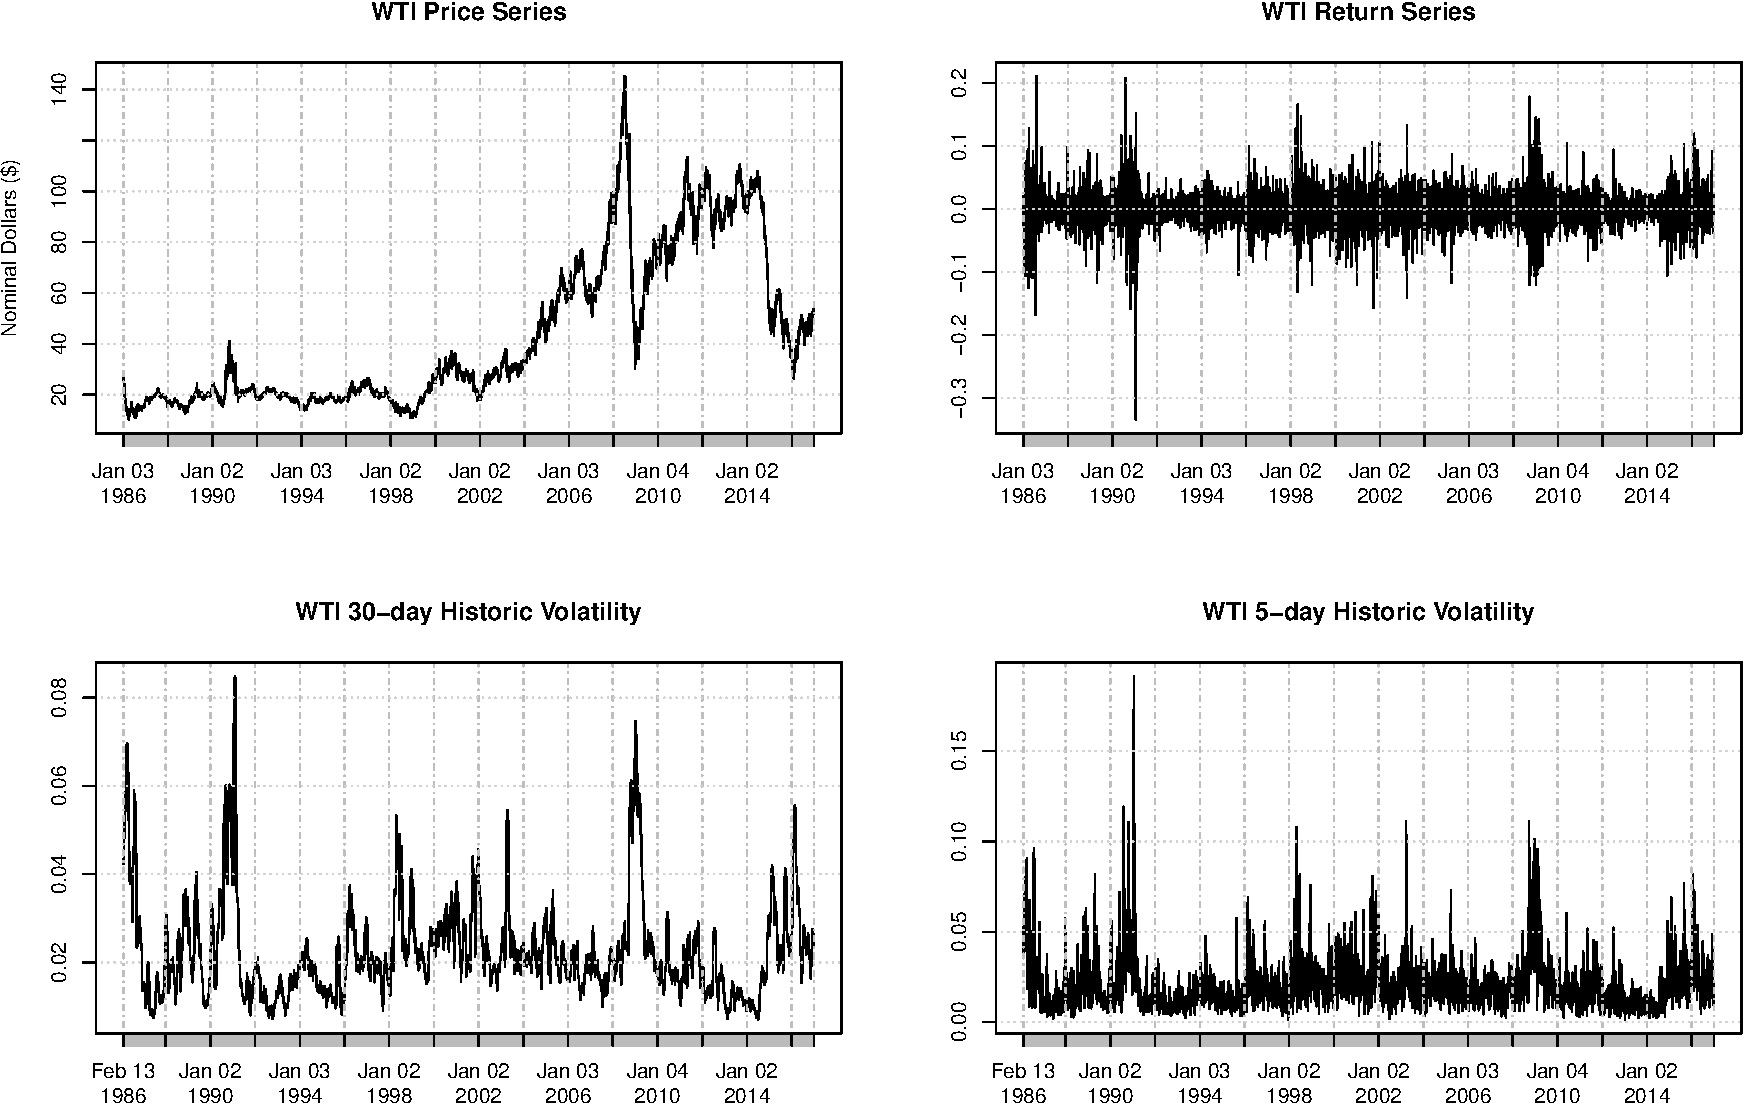
\includegraphics{Figs/unnamed-chunk-4-1.pdf}
\caption{Price level, return, and volatility series plots of WTI spot
oil prices.}
\end{figure}

A seen in Figure 1, most of the series from 1986 through 2004 contains
prices between \$10/barrel and \$40/barrel. This results in a price
series with a skewness value 0.98 and a long right tail (Figure 2), with
most prices being around the series median of \$28 per barrel. The
return series exhibits fatter tails and a narrower center than a normal
distribution of the same descriptive parameters. The kurtosis value of
the return series is 13.52. Returns with excess kurtosis compared to
normally distributed returns is a common characteristic in financial
time series. This indicates that most returns are very close to the mean
return, but some returns are dispersed very far from the mean.\\
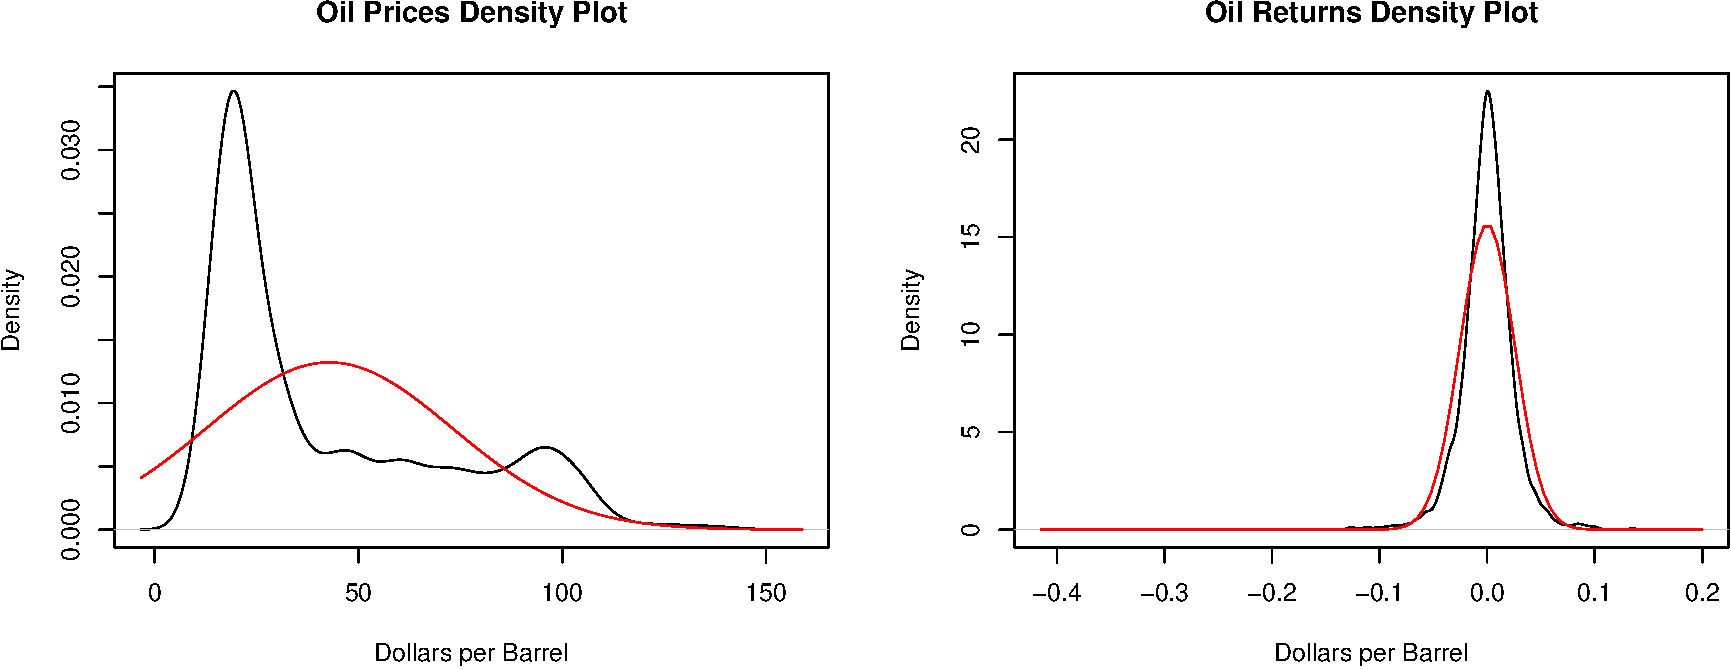
\includegraphics{Figs/unnamed-chunk-5-1.pdf}

\subsection{Autocorrelations}\label{autocorrelations}

Autocorrelations

\begin{figure}[htbp]
\centering
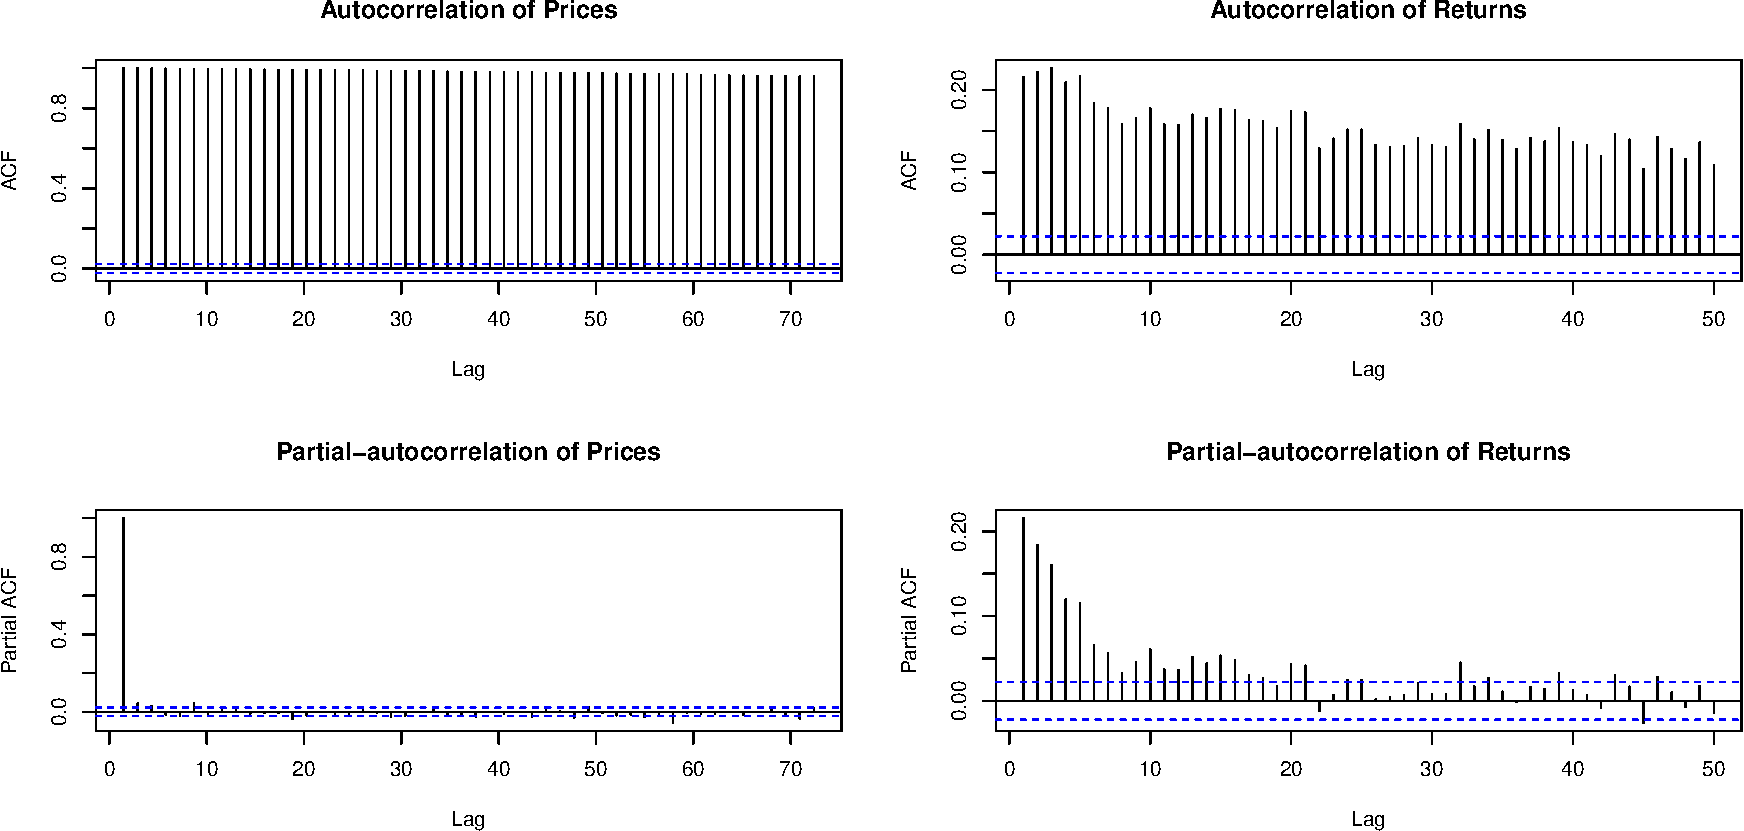
\includegraphics{Figs/unnamed-chunk-6-1.pdf}
\caption{Autocorrelation plots for prices and returns.}
\end{figure}

\section{Price-Volatility Regression
Analysis}\label{price-volatility-regression-analysis}

Relating price level and the measures of volatility at each time in the
series is a simple exploration of the research problem. The covariance
and correlation measures of vectors representing price versus returns,
30-day, and 5-day historic volatility indicate a weak, negative
relationship (Table 2). However, the unscaled return series indicates a
stronger positive covariance and correlation with the price series.

\begin{longtable}[]{@{}lrr@{}}
\caption{Covariance and correlation of price level and returns, 30-day,
and 5-day historic volatility.}\tabularnewline
\toprule
& Covariance & Correlation\tabularnewline
\midrule
\endfirsthead
\toprule
& Covariance & Correlation\tabularnewline
\midrule
\endhead
Return Series & 0.0102677 & 0.0134110\tabularnewline
Unscaled Return Series & 12.0871446 & 0.4393373\tabularnewline
30-day Historic Volatility & -1.0525476 & -0.1860878\tabularnewline
5-day Historic Volatility & -0.8388984 & -0.1123822\tabularnewline
\bottomrule
\end{longtable}

In quantitative finance, a process where volatility scales with price is
a lognormal process. When volatility is independent of price, the
process is normal (Ho and Lee, 2003). Regression of the price level and
squared returns is identified as the method of distinguishing lognormal
from normal processes in the literature. Figure 4 shows scatter plots of
the two return series and two historic volatility measures fitted with a
linear regression model.

\begin{figure}[htbp]
\centering
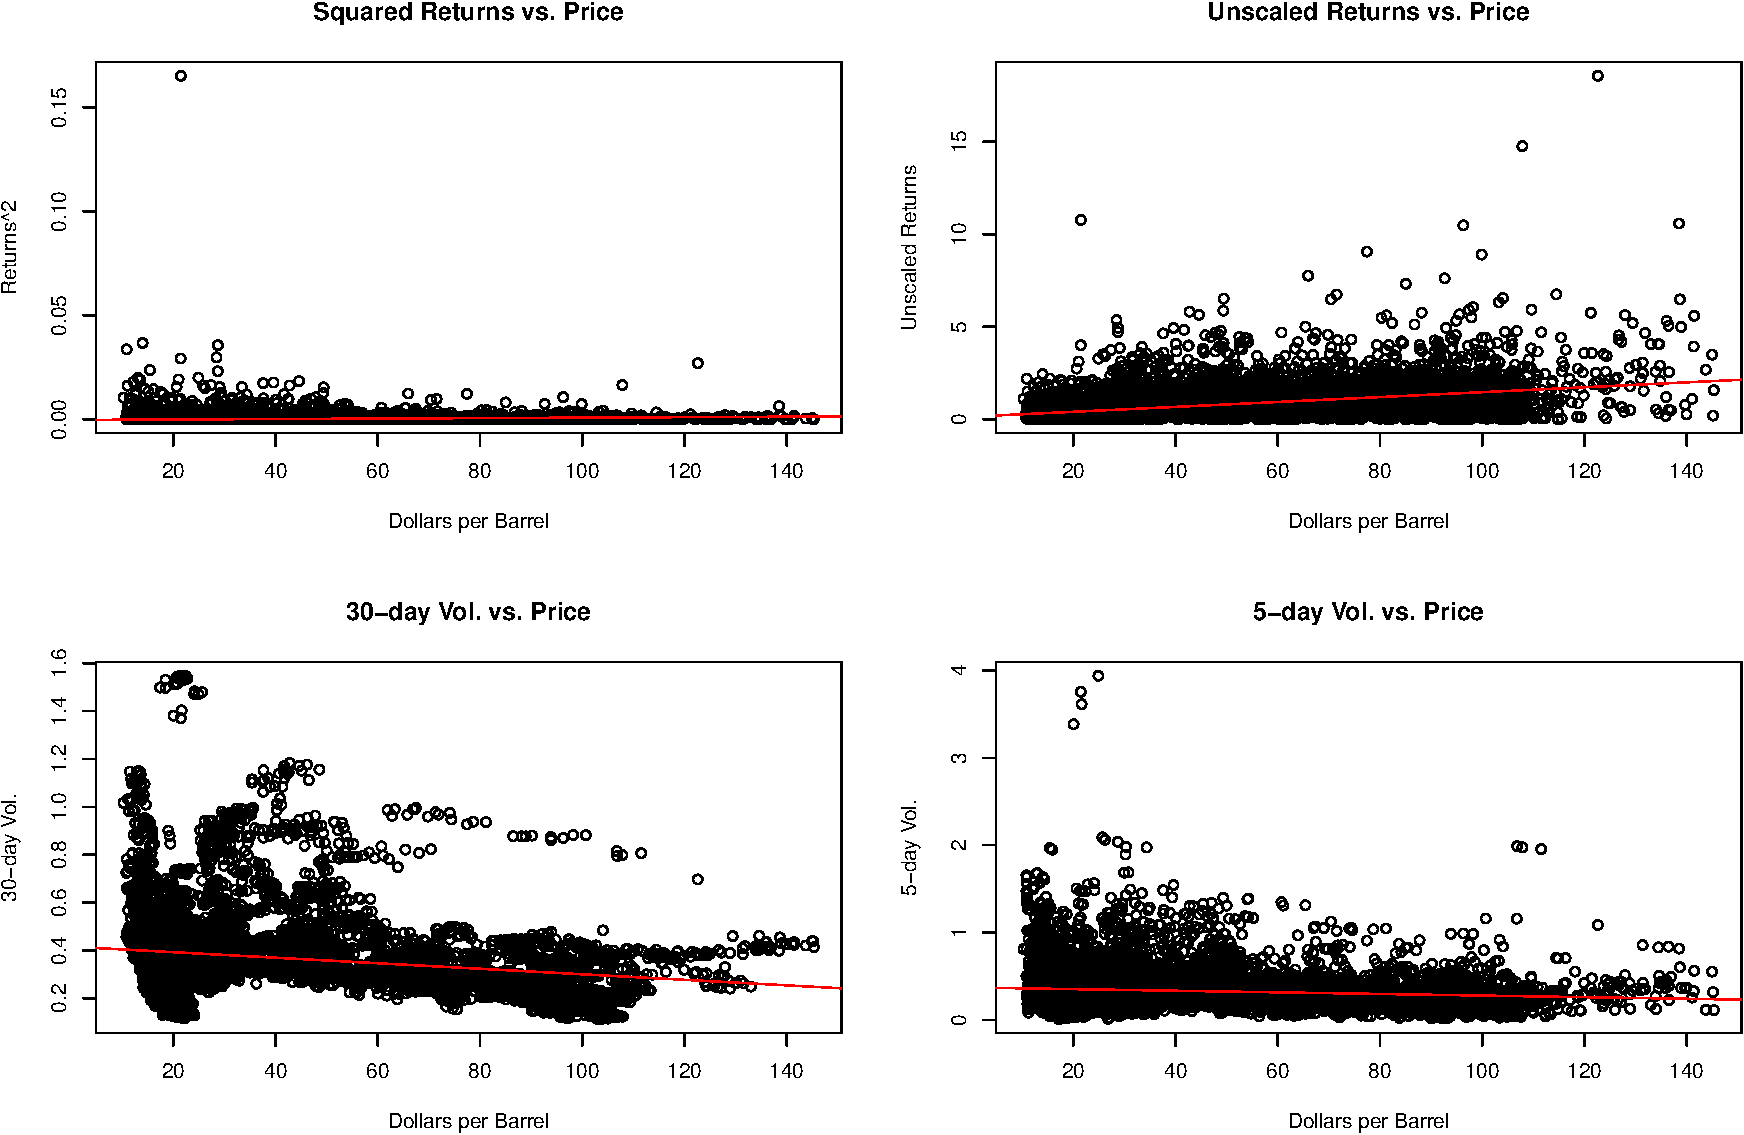
\includegraphics{Figs/unnamed-chunk-8-1.pdf}
\caption{Scatterplots with a linear model relating spot oil price with
returns, 30-day, and 5-day historic volatility.}
\end{figure}

The case of 30-day historic volatility indicates a negative relationship
between price level and volatility. However, this result appears to be
due to a cluster high volatility around \$20 per barrel, creating a
leverage point. Residual analysis indicates that this is not a good
relationship to model with linear regression.

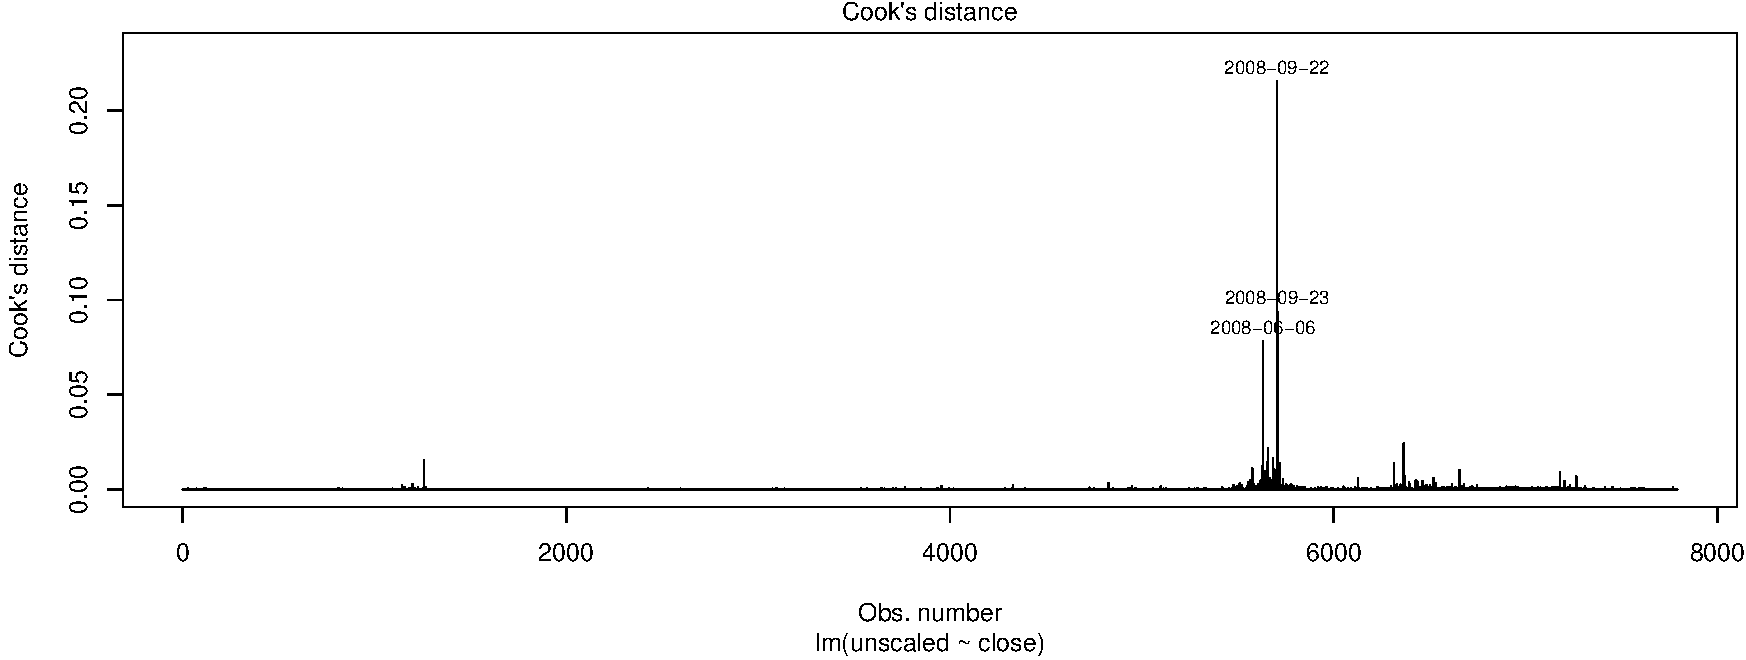
\includegraphics{Figs/unnamed-chunk-9-1.pdf}
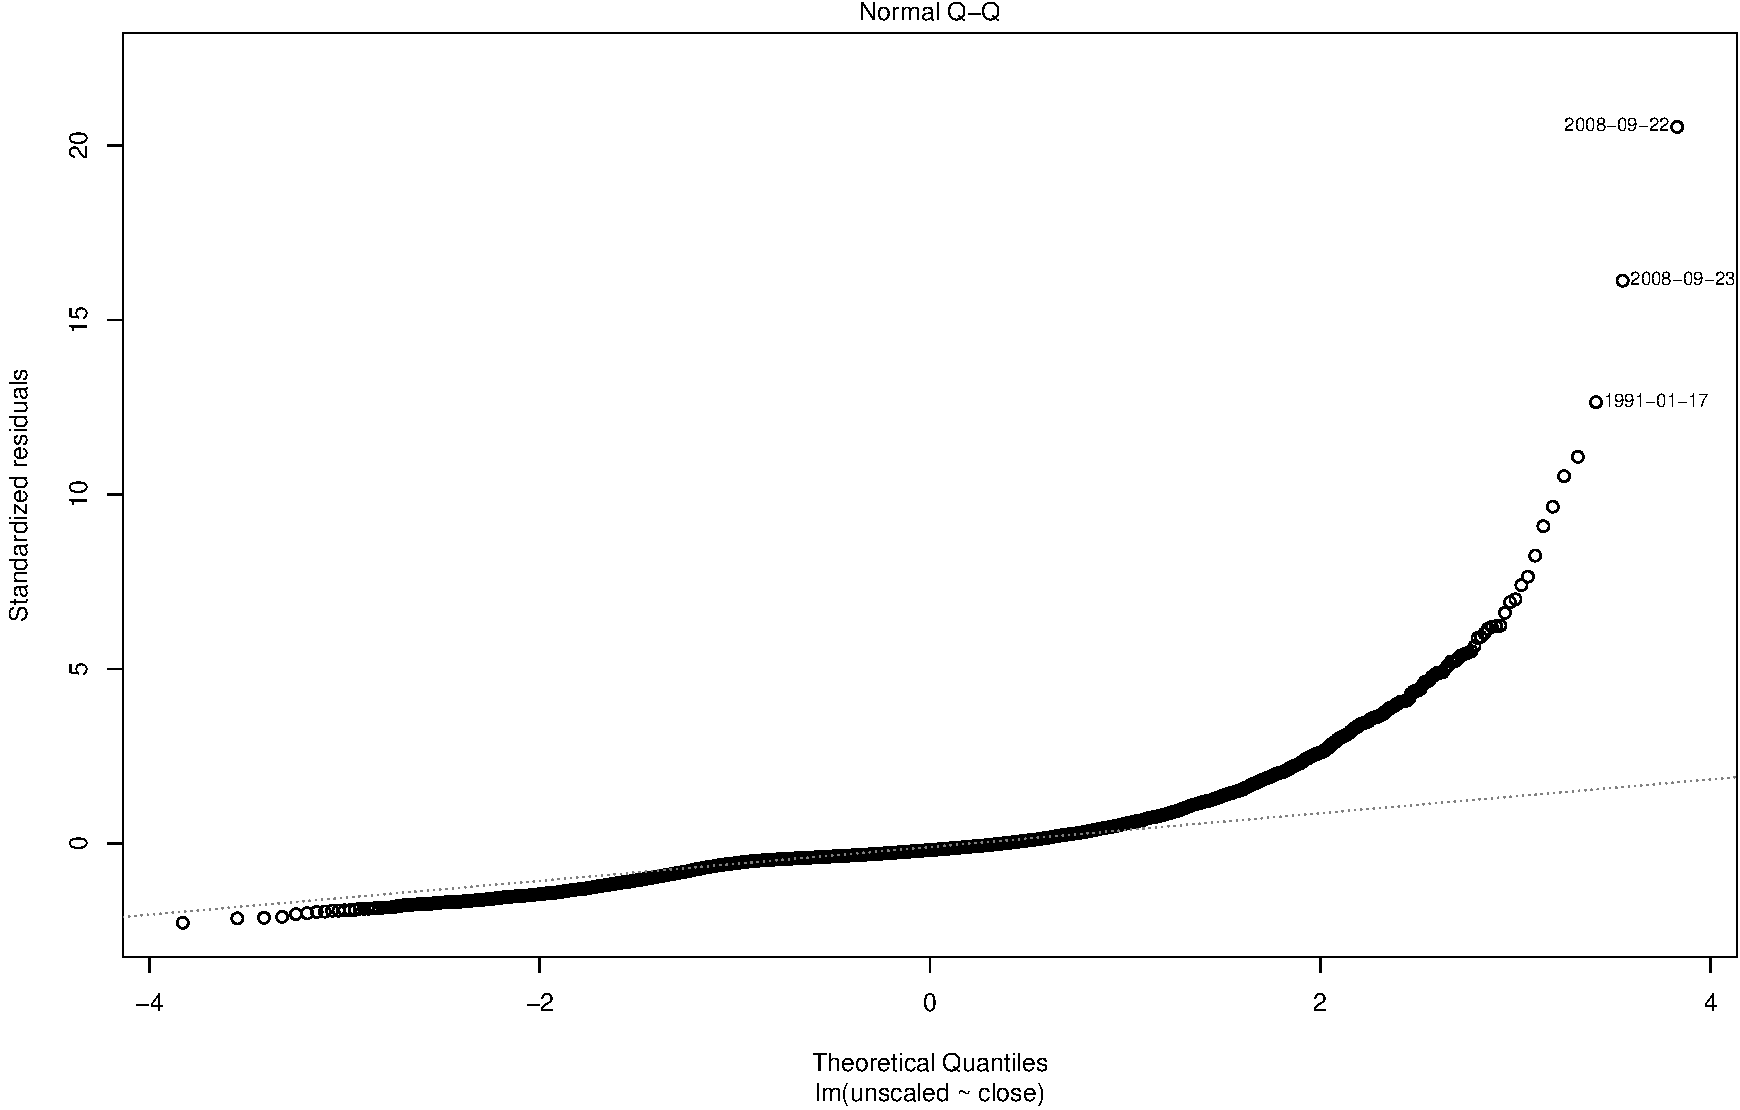
\includegraphics{Figs/unnamed-chunk-9-2.pdf}
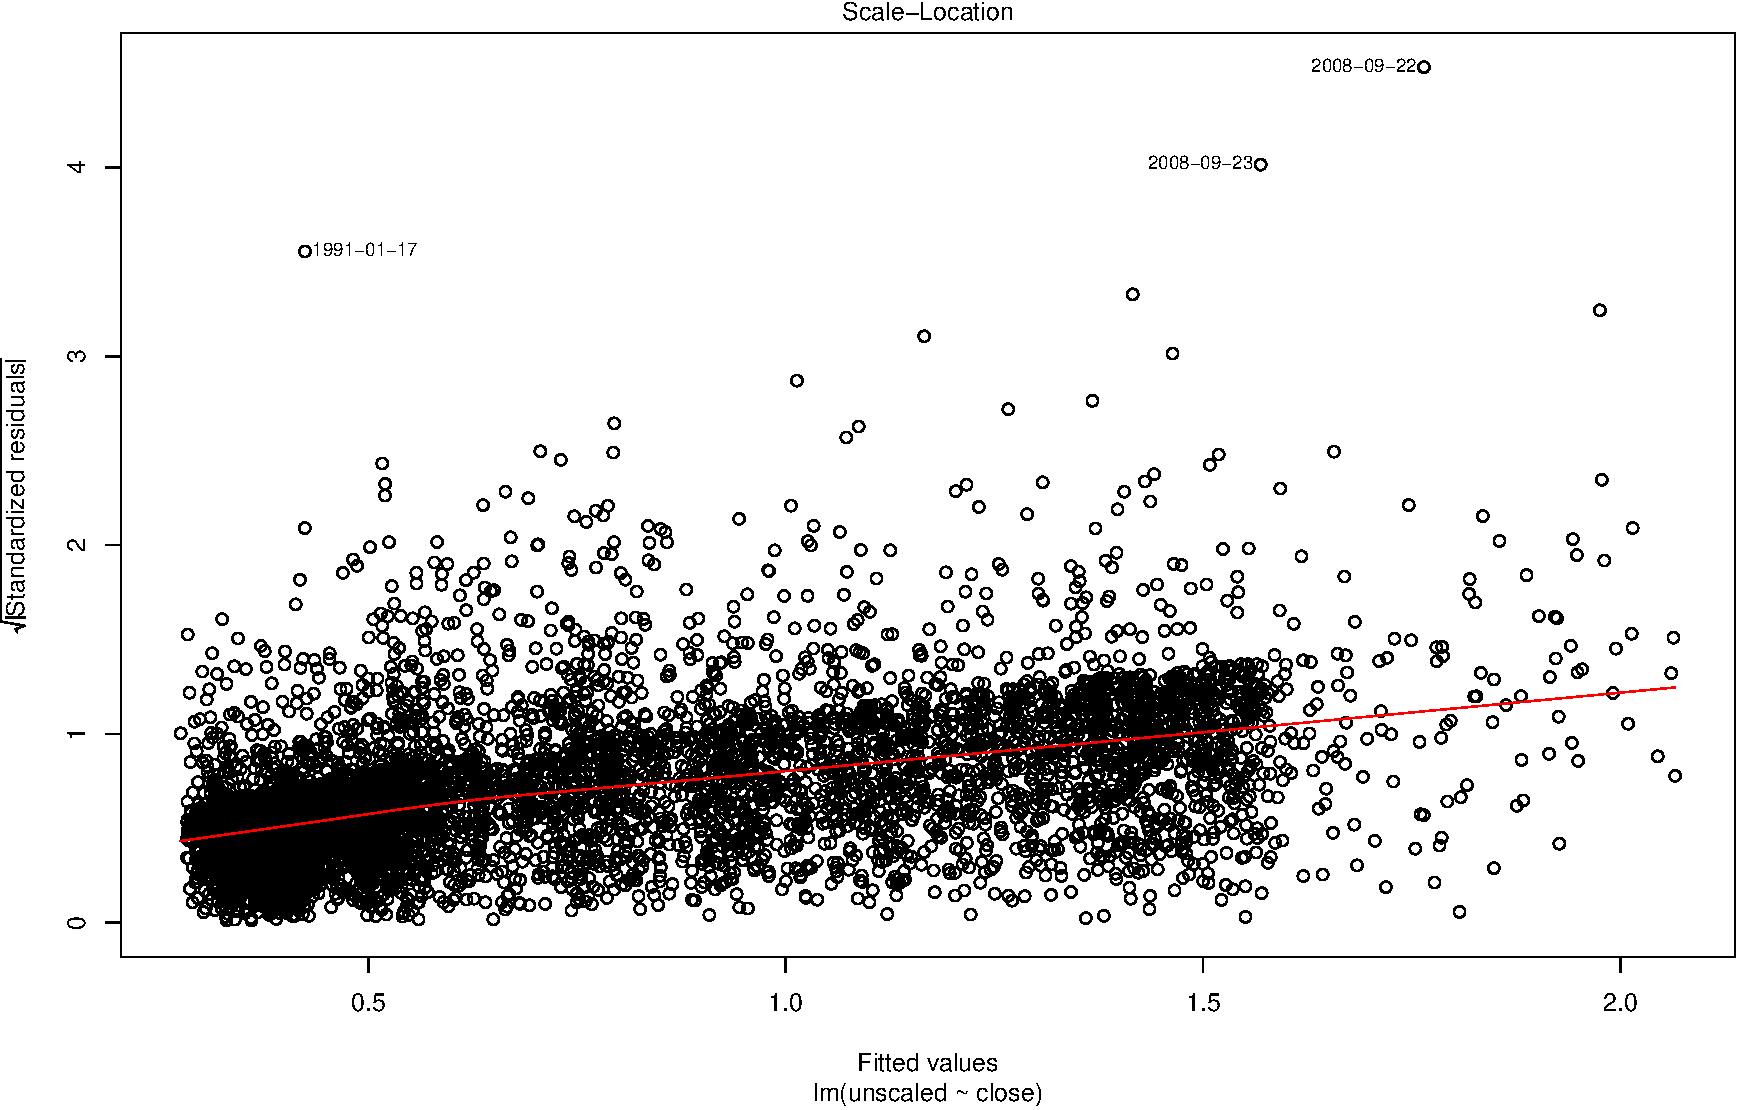
\includegraphics{Figs/unnamed-chunk-9-3.pdf}
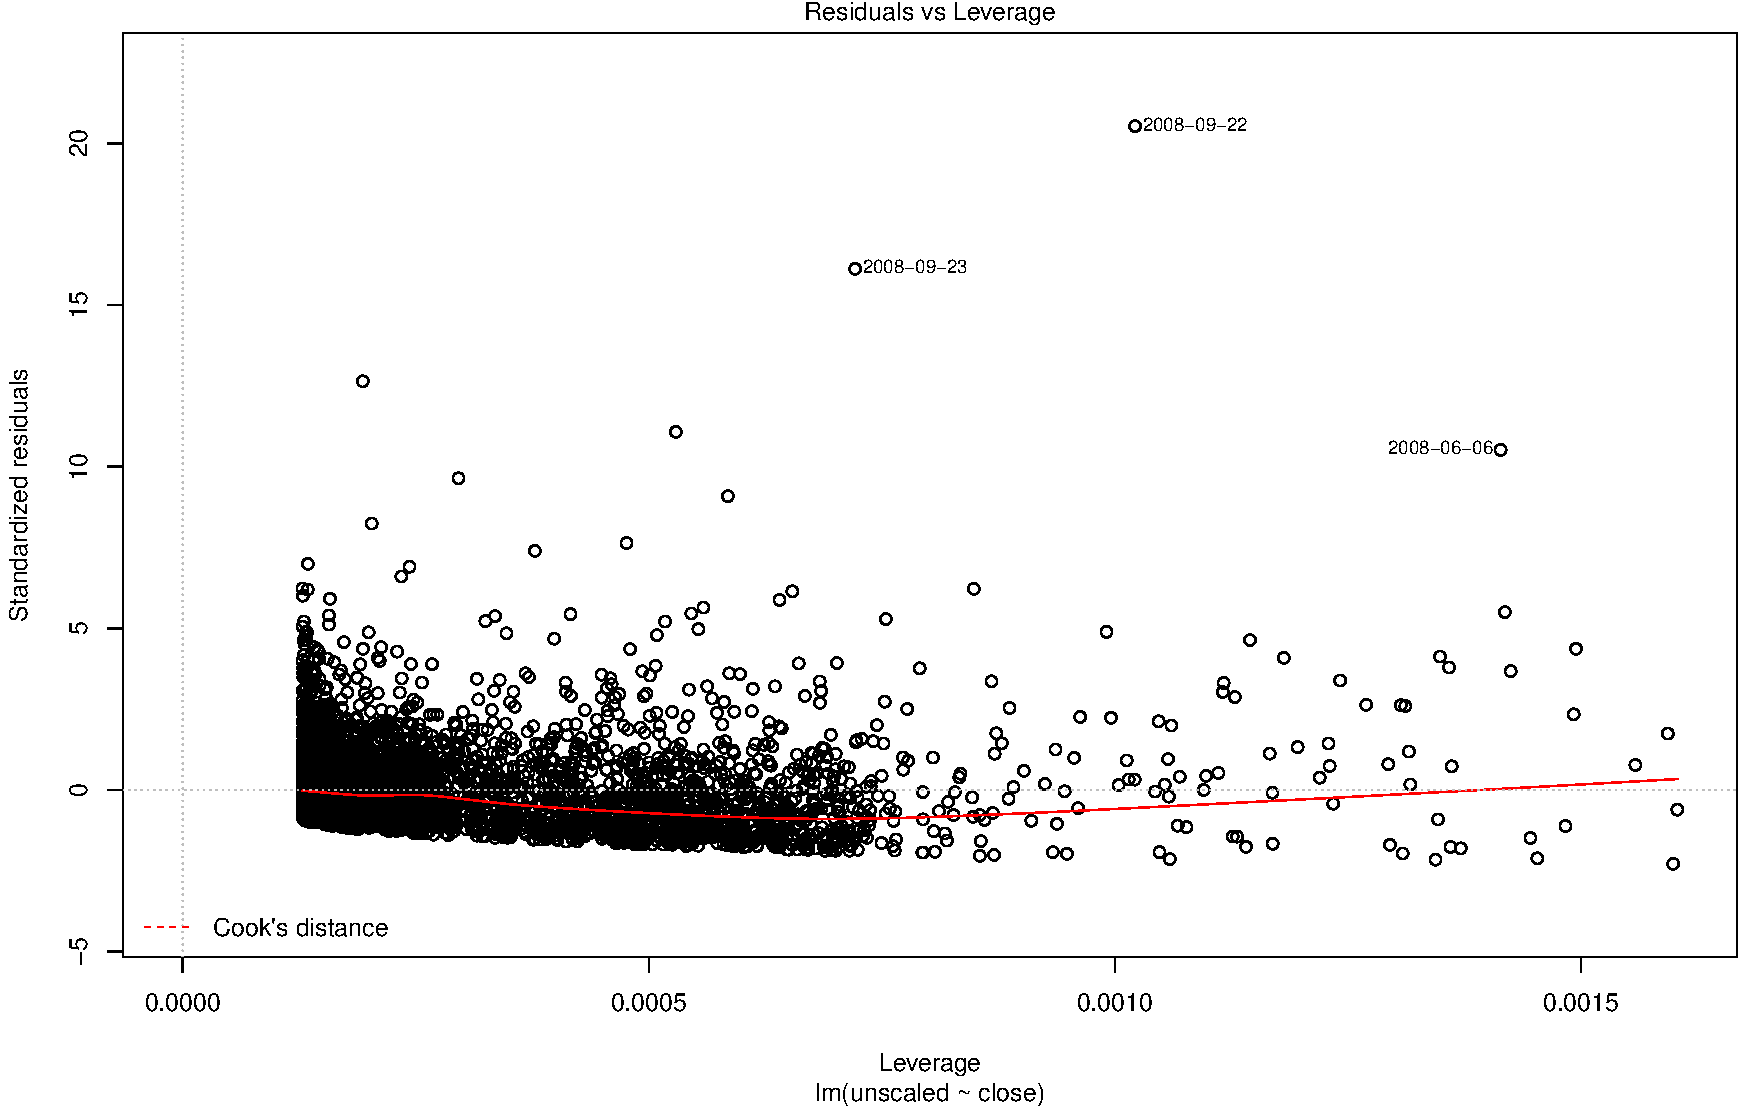
\includegraphics{Figs/unnamed-chunk-9-4.pdf}

As seen in Figure 1, nominal oil prices have spent time as high as \$145
per barrel. However, the majority of the time series is far lower, with
a median price of \$28 per barrel. This means that the dataset is
unbalanced and higher price levels represent a smaller portion of the
dataset. In addition, oil price (and financial time series in general)
exhibits volatility clustering. Therefore, it is anticipated that this
simple regression model based on price and volatility is not the best
possible solution to the question of characterizing the dependency of
volatility on price. A second time series was created by limiting WTI
prices to the January 3, 1998 through December 31, 2016. This results in
a distribution that, while significantly different than the normal
distribution, is more evenly distributed across the price range from
\$10.82 per barrel to \$145.30 per barrel (Figure 5).

Given the ever evolving economic, political, and technological landscape
affect commodity prices, there is some tradeoff between looking at a
large historic price record, which covers a larger data set of possible
system states (and higher statistical power), and limiting to a more
recent price record, which more fully represents the system in its
current state. However, the linear models relating price level to
returns and volatility resulting from the recent time series does not
differ much from using the full data set. In general there is a weak,
negative correlation between volatility and price, and a weak positive
correlation between returns and price.

This simple method of exploring the relationship between price level and
volatility does not provide a satisfactory explanation of whether we can
expect more volatility, indicating more commodity system uncertaintly,
at high price levels. Volatility in financial time series tend to
cluster. Typically, some event (called a ``shock'') occurs which results
in an extremely high price movement. These are the large noticeable
movements in the return series (Figure 1). Subsequent returns are also
of higher magnitude than the typical return size, but taper off over
time, eventually returning to a value close to the average return for
the price series. This is referred to as volatility clustering, and
indicates heterosketasticity in the variance component of a time series.
This violates the assumption in the most frequently used time series
model, the autoregressive integrated moving average (ARIMA) model.

These results using simple linear regression models to study how daily
returns and historic volatility relate to price level may not adequately
deal with this time-varying variance structure. If, for a given price
level, we have a price shock, we expect the volatility to return back to
its normal level. So at that price level we may have relatively few
measurements indicating high volatility, resulting in regression models
heavily weighted towards the baseline level of volatlity. This ``one to
one'' view of the price level - volatility relationship leaves the
question open as to whether we can anticipate more volatility or larger
price shocks at higher price levels.

\section{Comparing Volatility across Price
Regimes}\label{comparing-volatility-across-price-regimes}

In order to capture the volatility dynamics of the WTI price series,
including volatility clustering and changes in base price, change point
detection was used to break the series into price regimes. Change point
detection aims to detect the point or points where the statistical
properties of a sequence of observations change (Killick and Eckley,
2014). Change point detection was used to estimate changes in the oil
price mean throughout the period of record using the Pruned Exact Linear
Time (PELT) algorithm (Killick et al. 2012). The time series between
these changepoints represent ``price regimes'' (i.e.~time series between
changepoints) which have generally similar mean oil price compared to
the entire record.

Changepoint detection proceeds by minimizing a cost function over
possible locations and number of changepoints. The cost function:

\begin{verbatim}
## 
##  Fligner-Killeen test of homogeneity of variances
## 
## data:  wti.regimes.ret$returns and wti.regimes.ret$regime
## Fligner-Killeen:med chi-squared = 587.38, df = 14, p-value <
## 2.2e-16
\end{verbatim}

\begin{verbatim}
## [1] "statistic" "parameter" "p.value"   "method"    "data.name"
\end{verbatim}

The Fligner-Killeen test of homogeneity of variances determines if it is
appropriate to reject the null hypothesis that the variances between
each regime are the same. This test was chosen due to it's suitability
for non-normal data. The chi-squared value of the test was 587.38 and
the p-value was 0, indicating it is appropriate to conclude the
variances across the regimes are different.

Then, the standard deviation of the prices within a regime was compared
to the median price of the regime. The resulting dataset describing the
regimes were then modeled using linear regression. The resulting model
indicates a slope of 0.08, meaning that for every dollar increase in the
median price of a price regime, we expect an increase in the standard
deviation of that regime of 0.08. This model has an adjusted r-squared
value of 0.45.

\begin{longtable}[]{@{}lrrrr@{}}
\caption{Linear regression resulting from price as the predictor
variable and regime variance as the response variable.}\tabularnewline
\toprule
term & estimate & std.error & statistic & p.value\tabularnewline
\midrule
\endfirsthead
\toprule
term & estimate & std.error & statistic & p.value\tabularnewline
\midrule
\endhead
(Intercept) & 1.9666240 & 1.5125362 & 1.300216 &
0.2161068\tabularnewline
med & 0.0828545 & 0.0252947 & 3.275565 & 0.0060244\tabularnewline
\bottomrule
\end{longtable}

\begin{figure}[htbp]
\centering
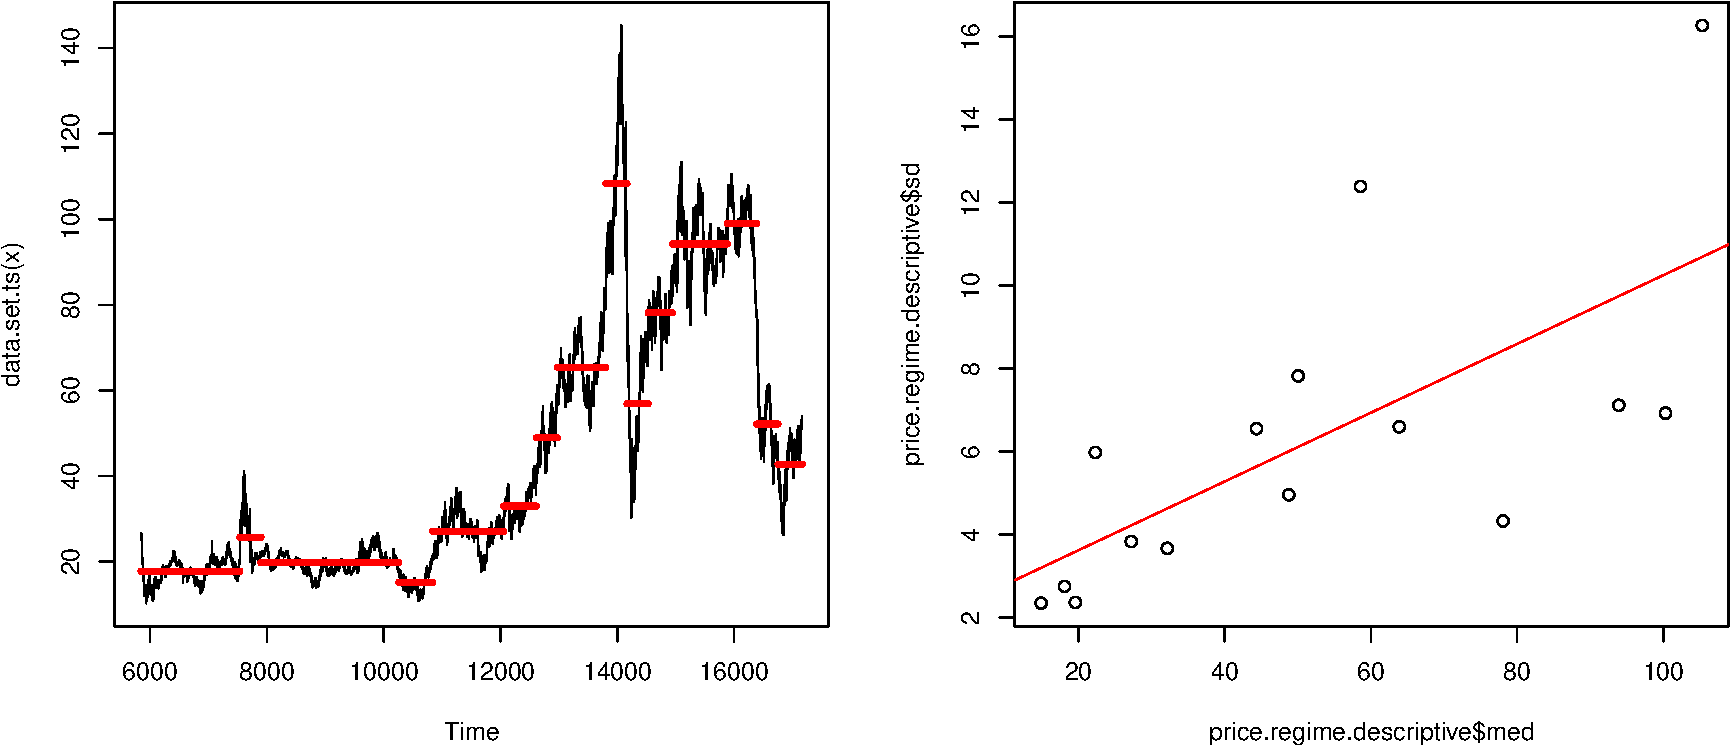
\includegraphics{Figs/unnamed-chunk-16-1.pdf}
\caption{Price regimes and linear model relating median oil price for
the regime to standard deviation within that price regime.}
\end{figure}

Analyzing the residuals of this model indicate some problems with the
fit. Namely, residuals are not evenly distributed and the model is
subject to suspected leverage point observations. This is typical in
linear models with small sample sizes.

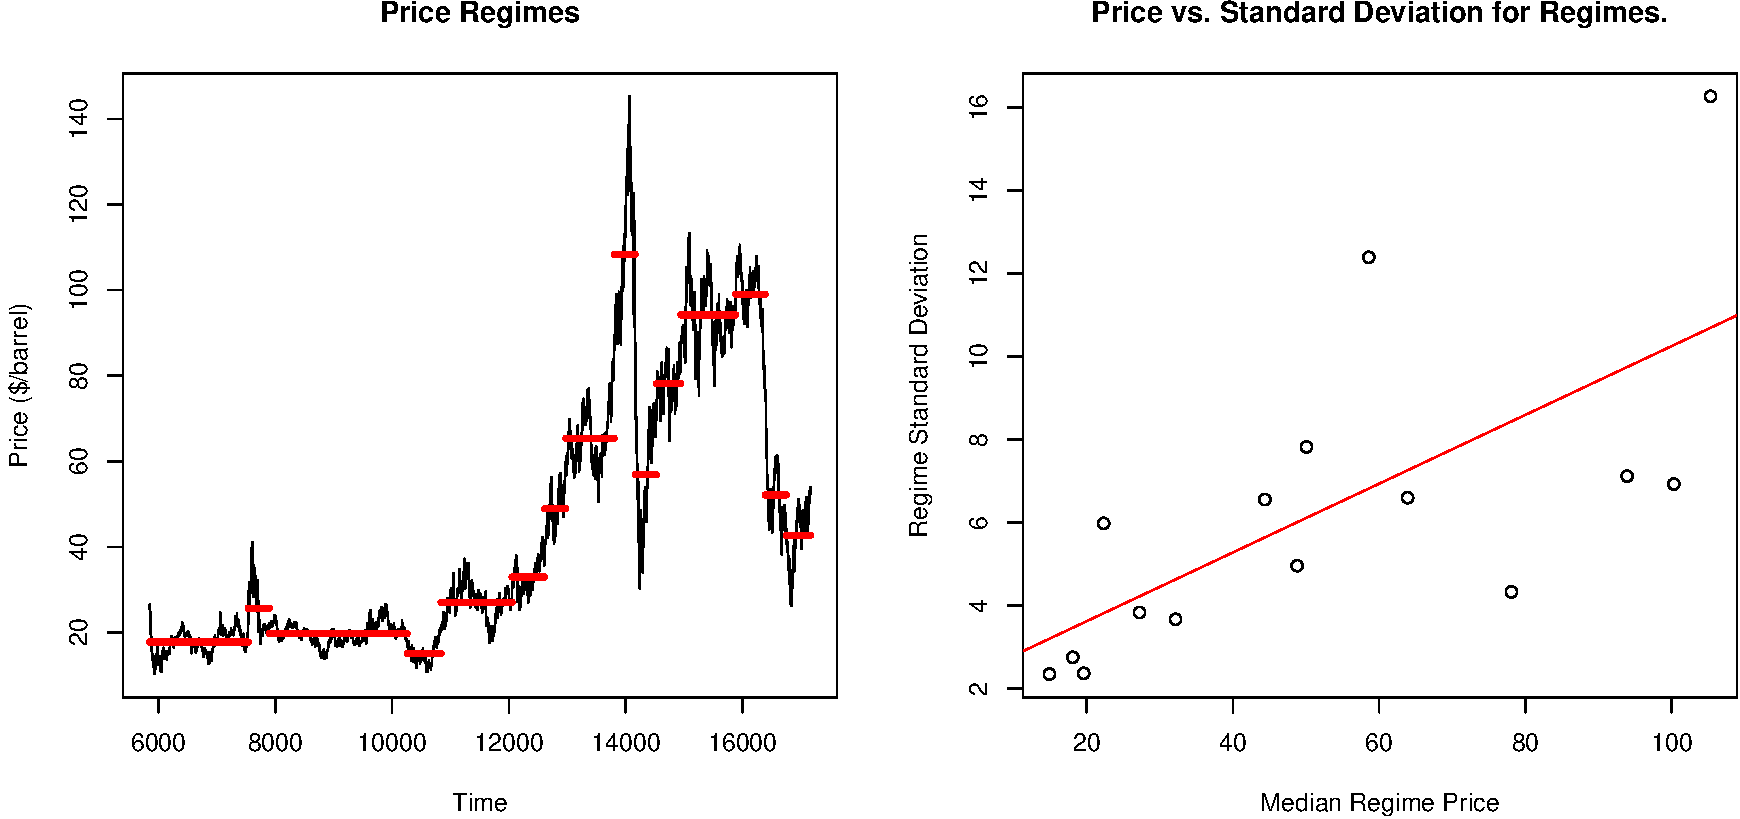
\includegraphics{Figs/unnamed-chunk-17-1.pdf}

In addition, this analysis was performed for the time series limited to
1998 - 2016, but this had little affect on the relationship between
price regime volatlitity.

This section's analysis using changepoint analysis to break the oil
price series into price regimes as defined by changes in the series mean
is highly dependent upon model parameters. The PELT change point
detection method identifies different regimes depending on the minimum
segment length and penalty parameters, and based on the section of the
time series used. An interactive Shiny App was created and may be access
in order to try different parameterizations of the change point model
and view the effects on the relationship between medial regime price and
standard deviation within that regime.

\section{Multivariate GARCH Model}\label{multivariate-garch-model}

Generalized AutoRegressive Conditional Heteroskedasticity (GARCH) models
attempt to model the variance component of a time series. It accounts
for asymetric, clustered variance

\section{Conclusion}\label{conclusion}

This analysis suggests that the question ``does oil price volatility
scale with price?'' requires further clarification to address.

\emph{Expected Returns at a Given Price Level} It is apparent from the
regression of unscaled returns to price level that we may expect returns
to increase linearly with increasing price. The linear model indicates
that for every one dollar increase in price, we may anticipate a 1.3
cent increase in expected returns. However, at

\(R_t = 0.013P_t+0.14\)

\begin{verbatim}
## 
## Call:
## lm(formula = unscaled ~ close, data = wti.combined)
## 
## Residuals:
##     Min      1Q  Median      3Q     Max 
## -1.8635 -0.3511 -0.1594  0.1853 16.7954 
## 
## Coefficients:
##              Estimate Std. Error t value Pr(>|t|)    
## (Intercept) 0.1394237  0.0161217   8.648   <2e-16 ***
## close       0.0132547  0.0003071  43.163   <2e-16 ***
## ---
## Signif. codes:  0 '***' 0.001 '**' 0.01 '*' 0.05 '.' 0.1 ' ' 1
## 
## Residual standard error: 0.8185 on 7789 degrees of freedom
## Multiple R-squared:  0.193,  Adjusted R-squared:  0.1929 
## F-statistic:  1863 on 1 and 7789 DF,  p-value: < 2.2e-16
\end{verbatim}

\emph{Scaled Volatiily}

\section{Acknowledgements}\label{acknowledgements}

\emph{I would like to thank John Kemp, Thompson Reuters energy
journalist, for posing the question investigated in this research paper.
In addition, I thank Tancred Lidderdale and Mason Hamilton from the U.S.
Energy Information Administration for additional information pertaining
to the question.}

\section{Bibliography}\label{bibliography}

Ghalanos, Alexios (2015). rmgarch: Multivariate GARCH models. R package
version 1.3-0.

Thomas S. Y. Ho and Sang Bin Lee, 2004. The Oxford Guide to Financial
Modeling: Applications for Capital Markets, Corporate Finance, Risk
Management and Financial Institutions. ISBN: 9780195169621


\end{document}
